%al posto di template.tex va messo il nome del file del livello superiore
\documentclass[../PianoProgetto.tex]{subfiles}

\begin{document}
%al posto di nome sezione va messo il nome della sezione appunto
\section{Pianificazione}

	Di seguito saranno elencate le durate e le caratteristiche di ogni fase. I tempi sono stati pensati per permettere uno slack sufficiente per abbassare i rischi relativi alle tempistiche.
	
	\subsection{Fase A: Analisi}
	
	\textbf{Periodo: dal 2015-11-23 al 2016-01-22}

	Questa fase comincia con la presentazione in aula delle "regole del progetto didattico". Essa termina con la scadenza della consegna della Revisione Dei Requisiti.

	Le sottofasi sono le seguenti:
	\begin{enumerate}
		\item Individuazione strumenti: In questa sottofase vengono scelti gli strumenti che saranno utilizzati per la stesura dei documenti, per il supporto e per il tracciamento dei requisiti;
		\item Norme Di Progetto: Dopo aver individuato gli strumenti si potrà procedere alla stesura del documento “Norme di Progetto v1.00”. Questo documento sarà utilizzato indipendentemente dal capitolato che sarà preso in appalto,
		\item Creazione documentazione: In questa fase sappiamo esattamente con cosa e in che modo dobbiamo scrivere un documento e possiamo iniziare la stesura dei documenti:
		\begin{itemize}
		\item Studio Di Fattibilità: Vengono valutati pro e contro di tutti i capitolati proposti e viene redatto il documento “Studio di Fattibilità v1.00”. Viene quindi scelto il capitolato da sviluppare;
		\item Analisi Dei Requisiti: Viene steso il documento “Analisi dei Requisiti v1.00”. Prima e durante la stesura di questo documento verranno organizzati degli incontri con il proponente per consolidare i requisiti stesi o per chiarire le idee sui requisiti da stendere;
		\item Piano Di Progetto: Si stende il documento “Piano di Progetto v1.00” per regolare le attività che il team dovrà svolgere;
		\item Piano Di Qualifica: Si redige il documento “Piano di Qualifica v1.00”;
		\item Glossario: viene incrementato il file “Glossario.xml” e steso in modo automatico il documento “Glossario v1.00”.
		\end{itemize}
	\end{enumerate}
		
		\subsubsection{Diagramma di Gantt – Fase A}
			\begin{figure}[!h]
				\centering
				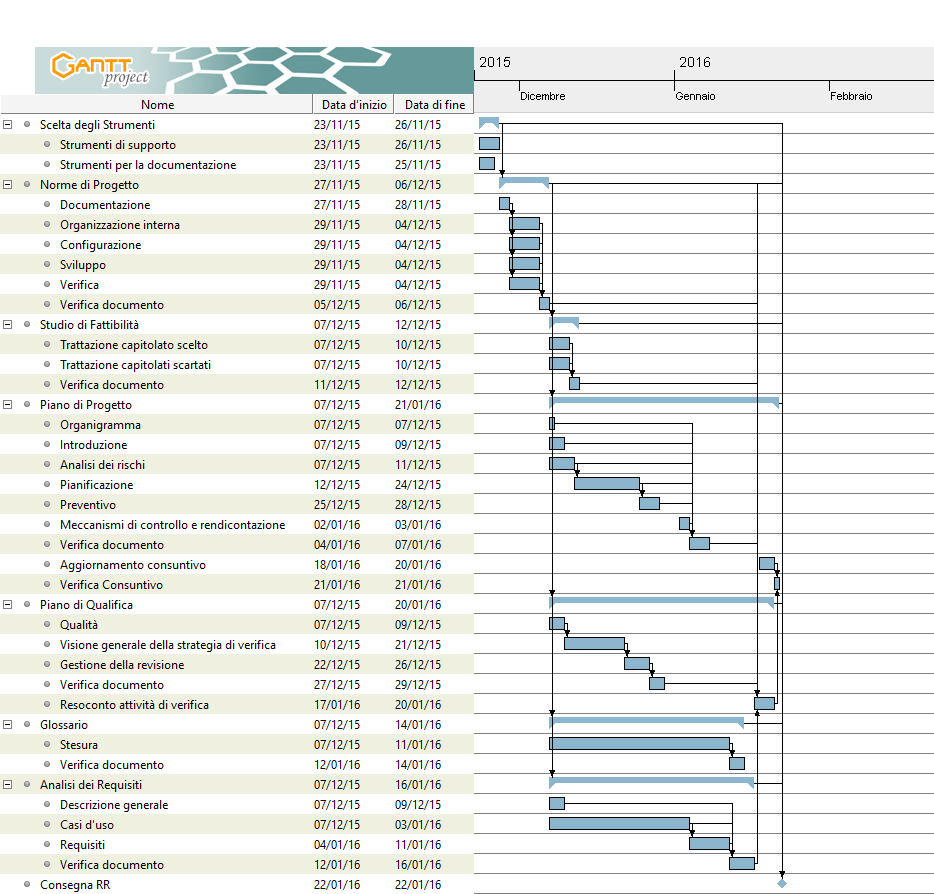
\includegraphics[width=\textwidth]{gantt_png/1-analisi}
				\caption{Gantt - Fase A}
				\label{fig:Gantt - Fase A}
			\end{figure}			
		
	\subsection{Fase AD: Analisi di Dettaglio}
		\textbf{Periodo: dal 2016-02-16 al 2016-02-22}

				Questa fase comincia al termine della Fase A. È caratterizzata da una nuova analisi di tutti i documenti redatti nella fase precedente e dalla correzione in base alle richieste e segnalazioni del Committente. Gli analisti provvedono all’individuazione di nuovi requisiti, alla correzione dei requisiti segnalati e si provvede all’incremento di tutti gli altri documenti.  Aggiornati i requisiti, si terrà un incontro con il Proponente per la loro verifica.
			
		\subsubsection{Diagramma di Gantt – Fase AD}
			\begin{figure}[!h]
				\centering
				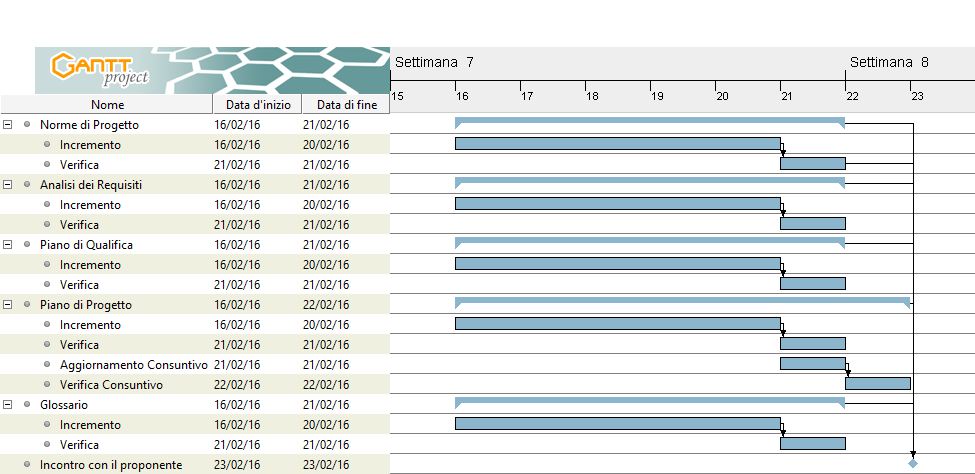
\includegraphics[width=\textwidth]{gantt_png/2-analisi_di_dettaglio}
				\caption{Gantt - Fase AD}
				\label{fig:Gantt - Fase AD}
			\end{figure}

	\subsection{Fase PA: Progettazione Architetturale}
		\textbf{Periodo: dal 2016-02-23 al 2016-03-20}
		
		Questa fase comincia con la fine della Fase AD e termina con l’incontro con il Proponente per mostrare l’architettura scelta. Le attività di questa fase sono:
		\begin{itemize}
			\item Norme di Progetto: Viene fatto un incremento alle norme per poter stendere il documento “Specifica Tecnica”. Viene successivamente fatta una verifica/validazione per fissare una baseline al documento che diventerà “Norme di Progetto v2.00”;

			\item Specifica Tecnica: Questa attività caratterizza la Progettazione Architetturale. Il Progettista stende la “Specifica Tecnica” che contiene le scelte progettuali, ad alto livello, che il progetto dovrà avere. Saranno quindi descritti quali design pattern implementerà, l’architettura generale del software, i principali flussi di controllo e il tracciamento dei requisiti;

			\item Glossario: Viene fatto un incremento al Glossario aggiungendo tutti i vocaboli che si ritiene importante siano inclusi. Viene successivamente fatta una verifica/validazione per fissare una baseline al documento che diventerà “Glossario v3.00”;

 			\item Piano di Qualifica: l’incremento consiste nell’aggiungere al documento “Piano di Qualifica v1.00” il dettaglio dell’esito della Revisione dei Requisiti e la parte della pianificazione dei test. Questa attività genererà, dopo una verifica e validazione, il file “Piano di Qualifica v2.00”;

			\item Piano di Progetto: l’incremento che sarà fatto al documento “Piano di Progetto” in questa fase consiste nell’apportare correzioni nella divisione delle attività e stillare il consuntivo di questo periodo. Dopo un’accurata verifica che fisserà una nuova baseline e la validazione il documento diventerà “Piano di Progetto v2.00”.
		\end{itemize}
		
		\subsubsection{Diagramma di Gantt – PA}
			\begin{figure}[!h]
				\centering
				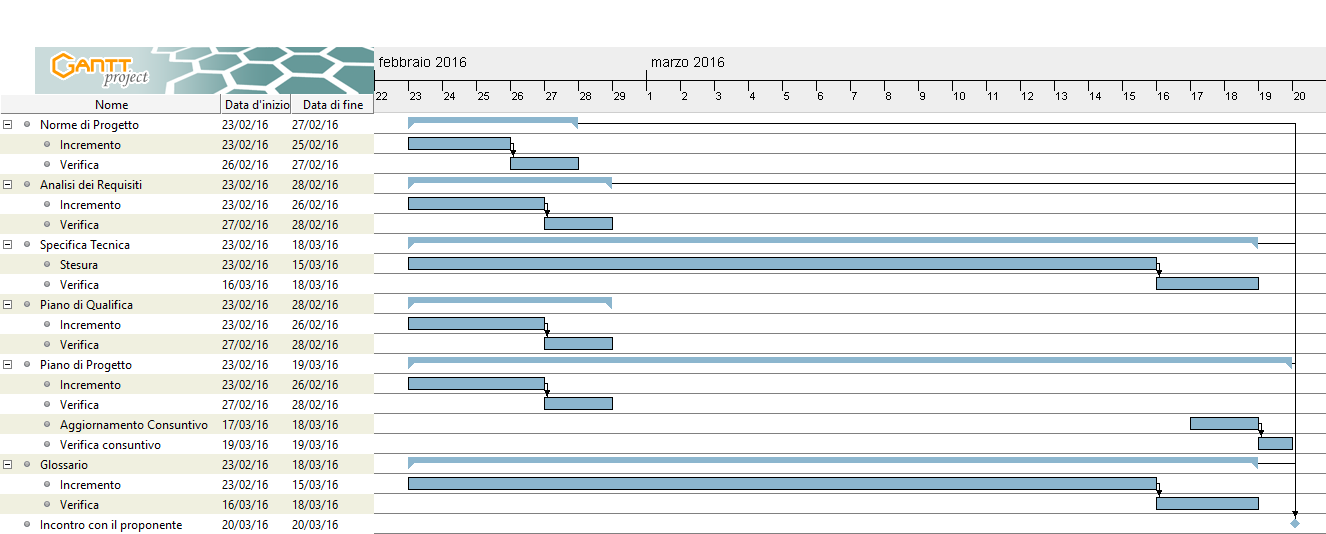
\includegraphics[width=\textwidth]{gantt_png/3-progettazione_architetturale}
				\caption{Gantt - Fase PA}
				\label{fig:Gantt - Fase PA}
			\end{figure}
						
	\subsection{Fase PDROB: Progettazione di Dettaglio e codifica dei Requisiti Obbligatori}
		\textbf{Periodo: dal 2016-03-21 al 2016-04-18}
		
		Questa fase comincia con la fine della Fase PA e termina con la consegna della Revisione di Progetto. Le attività di questa fase saranno le seguenti:
		\begin{itemize}
			\item Definizione di Prodotto: viene steso il documento “Definizione di Prodotto v1.00”. Esso definisce la struttura interna del sistema e le relazioni dei componenti del prodotto relativi ai requisiti obbligatori.

			\item Codifica: con quest’attività inizia lo sviluppo da parte dei programmatori dei requisiti obbligatori. Sarà dunque seguito quanto riportato nel documento “Definizione di Prodotto v1.00”;

			\item Esecuzione test: verranno eseguiti automaticamente tutti i test di unità previsti dal documento “Piano di Qualifica v 4.00”;

			\item Manuale Utente e Manuale Amministratore: comincia la stesura dei manuali che forniranno indicazioni agli utilizzatori del sistema.

			\item Incremento e Verifica Documenti: vengono eseguite modifiche ai documenti già scritti, se necessario.

			\item Glossario: vengono aggiunti al file “Glossario.xml” i vocaboli dei quali si ritiene necessaria una definizione formale. Alla fine di questa fase vieni quindi generato il documento “Glossario v4.00”.
		\end{itemize}
		
		\subsubsection{Diagramma di Gantt – PDROB}
			\begin{figure}[!h]
				\centering
				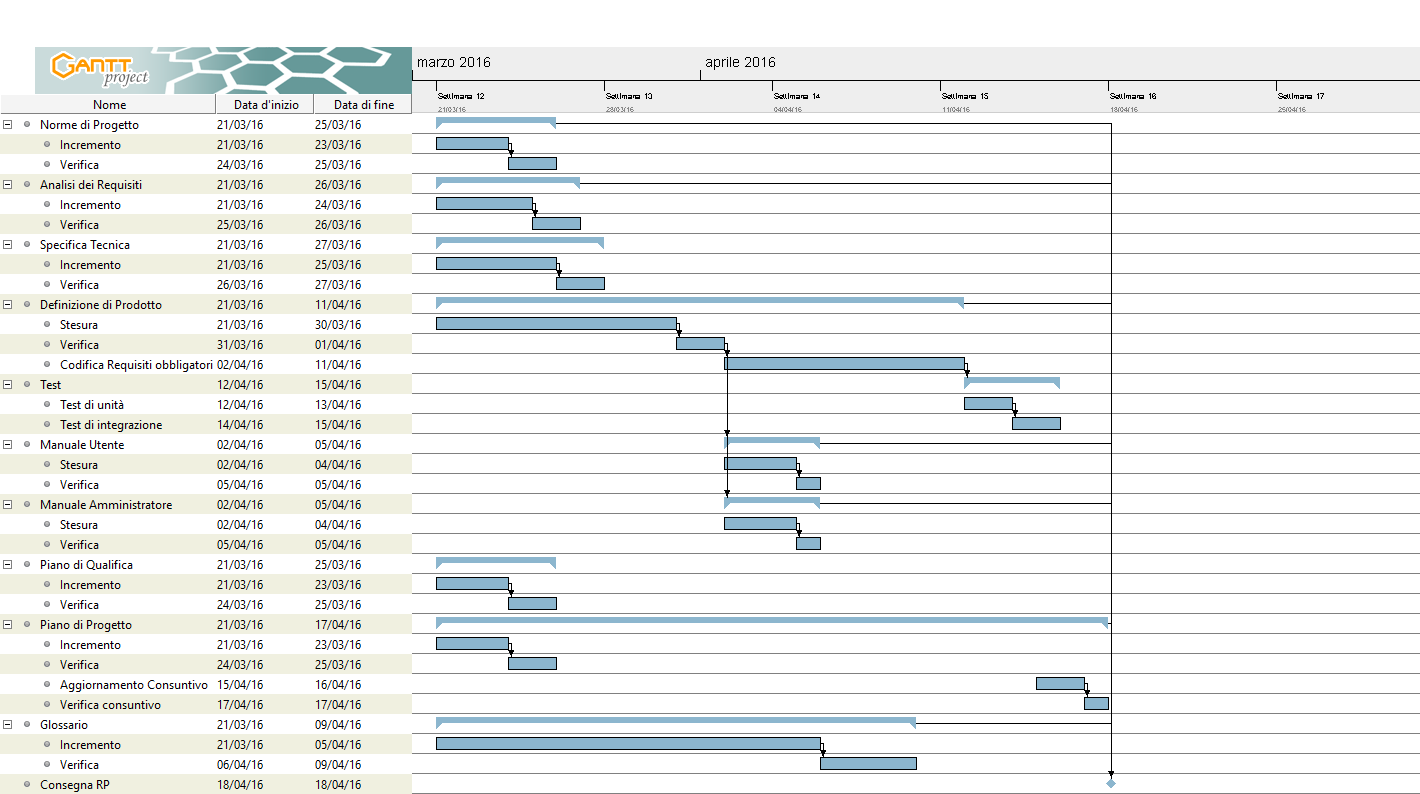
\includegraphics[width=\textwidth]{gantt_png/4-requisiti_obbligatori}
				\caption{Gantt - Fase PDROB}
				\label{fig:Gantt - Fase PDROB}
			\end{figure}
			
	\subsection{Fase PDRD: Progettazione di Dettaglio e codifica dei Requisiti Desiderabili}
		\textbf{Periodo: dal 2016-04-19 al 2016-05-09}
		
		Questa fase comincia con la fine della Revisione di Progetto e termina l’incontro con il proponente al fine di mostrare il prototipo con i requisiti obbligatori e desiderabili. Le attività di questa fase saranno le seguenti:

		\begin{itemize}
			\item Definizione di Prodotto: Viene steso il documento “Definizione di Prodotto v2.00”. Esso definisce la struttura interna del sistema e le relazioni dei componenti del prodotto relativi ai requisiti desiderabili.

			\item Codifica: con quest’attività inizia lo sviluppo da parte dei programmatori dei requisiti desiderabili. Sarà dunque seguito quanto riportato nel documento “Definizione di Prodotto v2.00”;

	 		\item Esecuzione test: verranno eseguiti automaticamente tutti i test di unità e integrazione previsti dal documento “Piano di Qualifica v 5.00”;

			\item Manuale Utente e Manuale Amministratore: Comincia la stesura dei manuali che forniranno indicazioni agli utilizzatori del sistema.

			\item Incremento e Verifica Documenti: Vengono eseguite modifiche ai documenti già scritti, se necessario.

			\item Glossario: Vengono aggiunti al file “Glossario.xml” i vocaboli dei quali si ritiene necessaria una definizione formale. Alla fine di questa fase vieni quindi generato il documento “Glossario v5.00”.
		\end{itemize}
		
		\subsubsection{Diagramma di Gantt – Fase PDRD}
			\begin{figure}[!h]
				\centering
				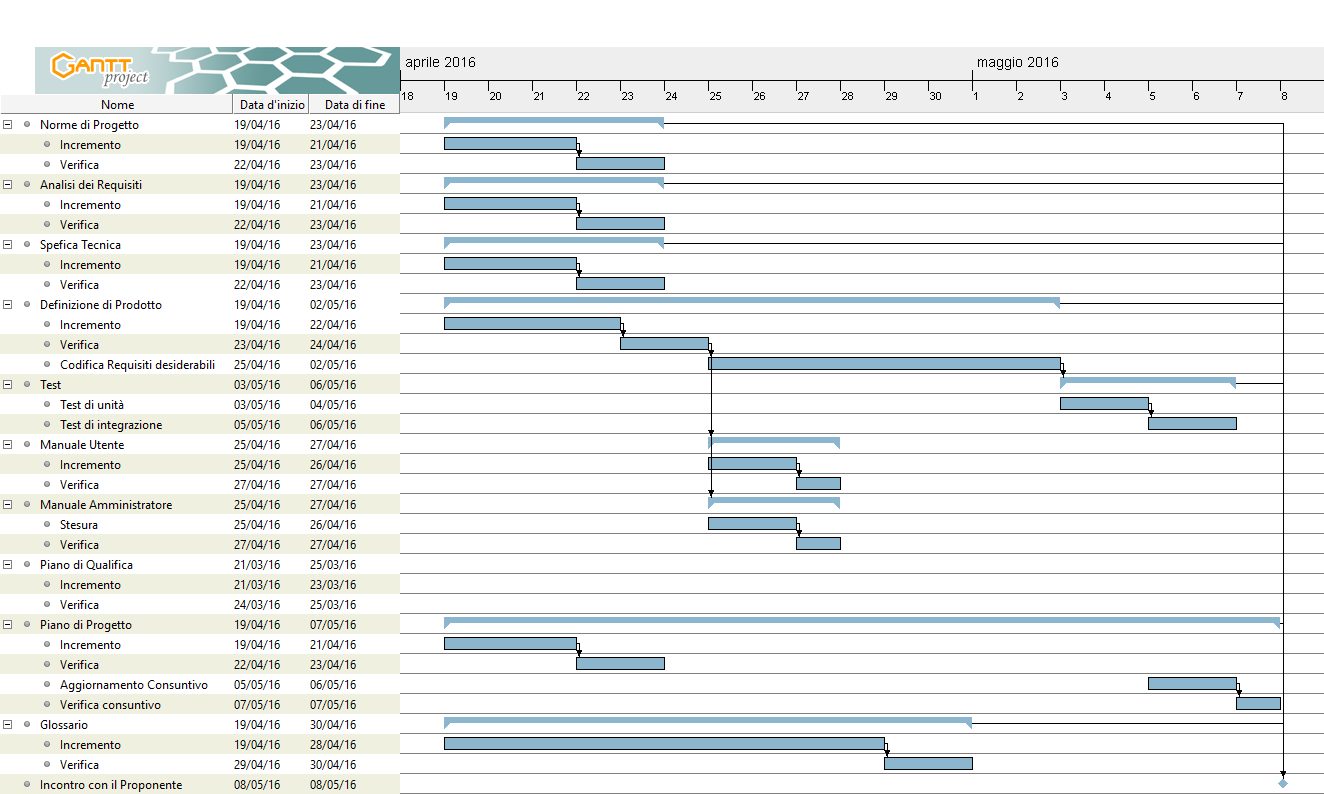
\includegraphics[width=\textwidth]{gantt_png/5-requisiti_desiderabili}
				\caption{Gantt - Fase PDRD}
				\label{fig:Gantt - Fase PDRD}
			\end{figure}
			
		
	\subsection{Fase PDROP: Progettazione di Dettaglio e codifica dei Requisiti Opzionali}
		\textbf{Periodo: dal 2016-05-10 al 2016-05-23}
		
		Questa fase comincia dopo la visione da parte del proponente del prototipo con i requisiti obbligatori e desiderabili e termina la consegna della Revisione di Qualifica.

		Le attività di questa fase saranno le seguenti:
		\begin{itemize}
			\item Definizione di Prodotto: viene steso il documento “Definizione di Prodotto v3.0”. Esso definisce la struttura interna del sistema e le relazioni dei componenti del prodotto relativi ai requisiti opzionali.

			\item Codifica: con quest’attività inizia lo sviluppo da parte dei programmatori dei requisiti opzionali. Sarà dunque seguito quanto riportato nel documento “Definizione di Prodotto v3.00”;

			\item Esecuzione test: verranno eseguiti automaticamente tutti i test di unità e integrazione previsti dal documento “Piano di Qualifica v 6.00”;

			\item Manuale Utente e Manuale Amministratore: comincia la stesura dei manuali che forniranno indicazioni agli utilizzatori del sistema.

			\item Incremento e Verifica Documenti: vengono eseguite modifiche ai documenti già scritti, se necessario.
			
			\item Glossario: vengono aggiunti al file “Glossario.xml” i vocaboli dei quali si ritiene necessaria una definizione formale. Alla fine di questa fase vieni quindi generato il documento “Glossario v6.00”.
		\end{itemize}
		
		\subsubsection{Diagramma di Gantt – PDROP}
			\begin{figure}[!h]
				\centering
				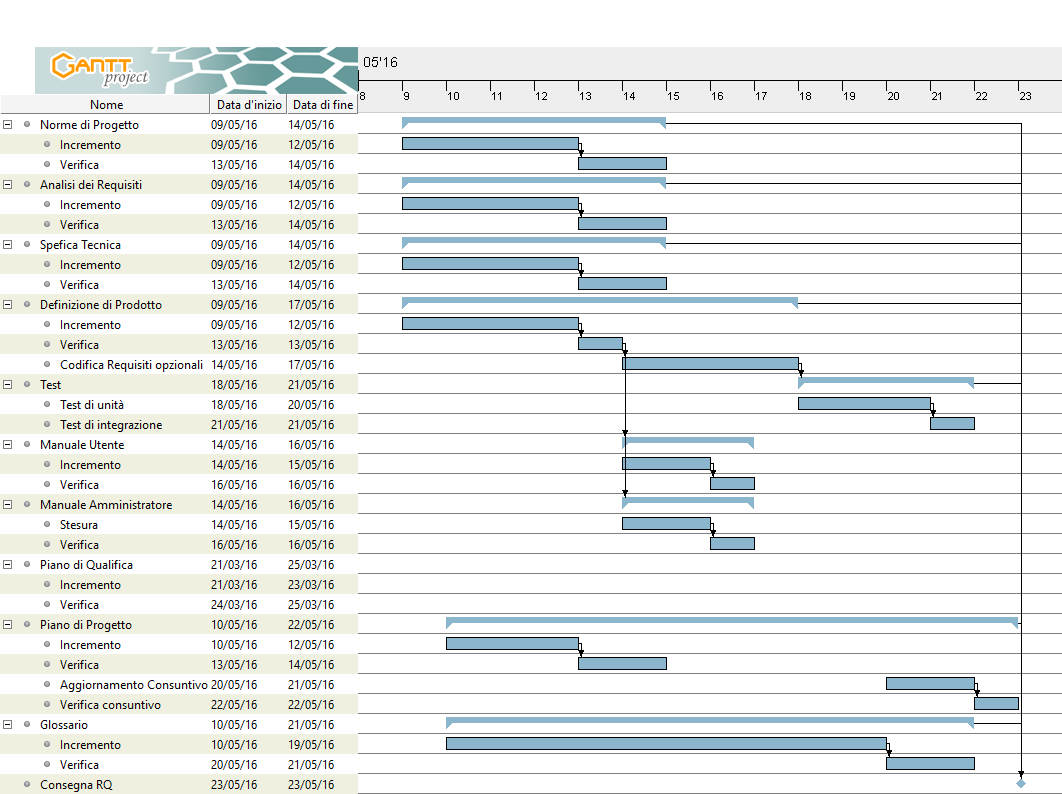
\includegraphics[width=\textwidth]{gantt_png/6-requisiti_facoltativi}
				\caption{Gantt - Fase PDROP}
				\label{fig:Gantt - Fase PDROP}
			\end{figure}
			
	
	\subsection{Fase V: Validazione}
		\textbf{Periodo: dal 2016-05-24 al 2015-06-17}
		
		Questa fase comincia con la consegna della Revisione di Qualifica e termina con la scadenza della consegna per la RA.

		\begin{itemize}
				\item Incremento e Verifica: se necessario verranno effettuati aggiornamenti ai vari documenti scritti;

				\item Validazione: viene verificato, attraverso tracciamento, di aver soddisfatto i requisiti presenti nel documento “Analisi dei Requisiti v1.00”;

				\item Esecuzione test: verranno eseguiti i test di sistema previsti dal documento “Piano di Qualifica v7.00”;

				\item Correzione bug: i bug rilevati verranno risolti;

				\item Collaudo: viene eseguito e completamente collaudato il sistema creato.
		\end{itemize}
		
		\subsubsection{Diagramma di Gantt – V}
			\begin{figure}[!h]
				\centering
				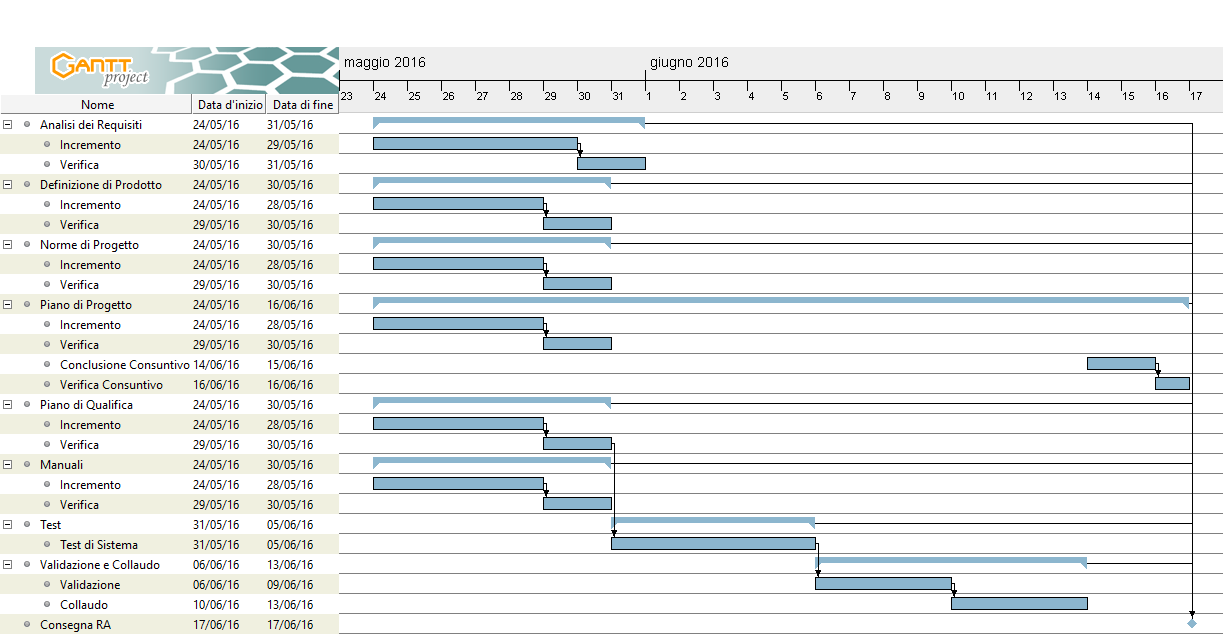
\includegraphics[width=\textwidth]{gantt_png/7-verifica}
				\caption{Gantt - Fase V}
				\label{fig:Gantt - Fase V}
			\end{figure}
			

\end{document}